\documentclass[12pt,a4paper]{amsart}
\usepackage[utf8]{inputenc}
\usepackage{amsmath}
\usepackage{amsfonts}
\usepackage{amssymb}

\usepackage[all,cmtip]{xy}

\usepackage{hyperref}

\usepackage{float}
\usepackage{subfig}


%\usepackage[dvipdfmx]{graphicx}
\usepackage{graphicx}
\usepackage{caption}
%\usepackage[nobysame, alphabetic]{amsrefs}
%\usepackage{here}
%\usepackage{showkeys}
\newcommand{\modif}{$\clubsuit$}
\newtheorem{thm}{Theorem}
\newtheorem{defn}[thm]{Definition}
\newtheorem{coro}[thm]{Corollary}
\newtheorem{prop}[thm]{Proposition}
\newtheorem{lem}[thm]{Lemma}
%\theoremstyle{definition}
\newtheorem{rmk}[thm]{Remark}
\newtheorem{cond}[thm]{Condition}

%CB defs
\def\rh{\phi_h}
\def\rv{\phi_v}

\def\HH{\mathbb{H}}
\def\GG{\mathbb{G}}
\def\dHH{\partial \mathbb{H}}
\def\hd{\hat{\delta}}
\def\ha{\hat{\alpha}}
\def\haa{\ha \cup \{\alpha^+,\alpha^-\}}

\def\im{\mathrm{Im}\,}
\def\re{\mathrm{Re}\,}
\def\oo{\HH / \Gamma_0(2)} 
\def\ooo{\HH / \Gamma_0(3)} 
\def\g2{\Gamma(2)}
\def\go2{\Gamma_0(2)}
\def\ah{\Gamma_0^t(2)}
\def\oot{\HH / \ah} 
\def\xx{\HH/\g2}


\def\ZZ{\mathbb{Z}}
\def\CC{\mathbb{C}}
\def\RR{\mathbb{R}}
\def\QQ{\mathbb{Q}}
\def\NN{\mathbb{N}}

\def\qqq{\mathbb{Q} \cup \{\infty\}}

\def\tt{\Sigma_{1,1}}

\def\fp{\mathbb{F}_p}
\def\aut{\text{Aut}(\F2)}
\def\glz{\mathrm{GL}(2, \ZZ)}
\def\slr{\mathrm{SL}(2, \ZZ)}
\def\slc{\mathrm{SL}(2, \CC)}
\def\slz{\mathrm{SL}(2, \ZZ)}

\def\lc{\mathcal{C}}

\def\oi{\Gamma.\{i\}}
\def\hp{\tilde{\mathcal{P}}}


\def\isom{\mathrm{isom}(\HH)}

\def\isomH{\text{isom}^+(\HH)}
\def\tr{\text{tr\,}}


\def\GI{\mathbb{Z}[i]}
\def\hc{\CC \setminus \GI}



\title{Pythagorean triples}

 % \author[Vlad]{Vlad Sergesciu}
\address{Institut Fourier 100 rue des maths, BP 74, 38402 St Martin d'H\`eres cedex, France}
\email{mcshane at univ-grenoble-alpes.fr}


\begin{document}

\maketitle

\section{Introduction}

A \textit{Pythagorean triple} is a triple of integers $(a,b,c)$ such
that $$a^2 + b^2 = c^2.$$
The most famous example is the so-called \textit{egyptian triple}
$(3,4,5)$ which is \textit{a priori} the ``smallest'' Pythagorean triple.	
The set of Pythagorean triples is infinite, and it is a classical problem to find all Pythagorean triples. 
It is useful to define the notion of \textit{primitive Pythagorean
triple}, which is a Pythagorean triple $(a,b,c)$ such that
the three integers have no common divisor greater than 1.
Evidently, any Pythagorean triple can be written as a multiple of a primitive Pythagorean triple.
In fact, the set of primitive Pythagorean triples 
forms what is
essentially (see below for a precise statement) a single orbit under the action of a group of transformations the orthognal group $O(2,1;\ZZ)$ on the Minkowski space $\mathbb{R}^{2,1}$.
This is because every Pythagorean triple is an integer point on the
\textit{light cone} of Minkowski space: 
$$ \{ (x,y,z) \in \mathbb{R}^3 \mid -x^2 - y^2 + z^2 = 0 \}.$$
We note that the ``smallest" integer point on the light cone is not
$(3,4,5)$, but rather $(1,0,1)$ or $(0,1,1)$.
Of course, these two points correspond to degenerate Pythagorean triangles i.e. triangles of area zero.

\section{Euclid's parameterization}


The Pythagorean triples that are relatively prime, called the
\textit{primitive triples}, have
the elementary and beautiful characterization as integers
due to Euclid:
$$(a,b,c) = (m^2 - n^2, 2mn, m^2 + n^2)$$
where $m$ and $n$ are coprime integers of opposite parity and $m > n > 0$.
Another way to think of this is
that $c$ factors over the Gaussian integers $\mathbb{Z}[i]$ 
as 
$$c = (m+ni)(m-ni),$$ 
where $m$ and $n$ are coprime integers of opposite parity,
that is exactly one is odd and the other is even
so it follows that:
\begin{itemize}
	\item $c= m^2 + n^2$ is odd,
	\item $a$ is the real part of the product 
	\item $b$ is the imaginary part of the product.
\end{itemize}
Note that $a$ and $b$ are, like $m$ and $n$, are of opposite parity.

More generally,  we have maps : 
$$(x,y)\in \RR^2 \mapsto z = x + iy \mapsto z^2 \mapsto (\Re z^2, \Im z^2,
|z^2|) = (a,b,c) \in \lc .$$
% where $z^2 = (m+ni)^2 = m^2 - n^2 + 2mni$.
The composition $p:(x,y) \mapsto (a,b,c)$ is a surjection 
since the system of equations below always has a solution
for $x,y \in \RR_+$:
\begin{eqnarray*}
2 x^2 &=& a + c, \\
2 y^2 &=&  c - a > 0.
\end{eqnarray*}
Further, the restriction of the map $p:(x,y) \mapsto (|a|,|b|,|c|)$
to the subset
$$\hp = \{(m,n) \in \ZZ^2, \gcd(m,n) = 1,  m+n \text{ odd}\}$$
is  a surjection onto the set of primitive Pythagorean triples.
Note that $\hp$ is a subset of the set of
\textit{primitive elements} of the group $\ZZ^2$.
The group of  integer
matrices $\Gamma = \slz$ acts on $\ZZ^2$,
it acts transitively on primitive elements of $\ZZ^2$,
so does not preserve the set $\hp$
however the principal congruence subgroup $\g2$ does.


\section{Hall matrices}


The set of polynomials with integer coefficients $\ZZ[X,Y]$ forms a free $\ZZ$-module.
There is a submodule freely generated by the polynomials
$$(X^2 - Y^2, 2XY, X^2 + Y^2).$$
The group $\Gamma(2)$ acts on this submodule by change of basis and we can
compute the matrices of the generators of $\Gamma(2)$ with respect
to this basis.
Since the basis satisfies the relation:
$$-(X^2 + Y^2)^2 +  (X^2-Y^2)^2 + (2XY)^2 = 0,$$
these matrices are elements of $O(2,1;\ZZ)$.


\section{Enumeration}

The problem of finding all primitive Pythagorean Triples
is equivalent to the problem of finding all the primitive elements
$(m,n)$ of the group $\ZZ^2$ 
that satisfy:
\begin{itemize}
	\item $n \geq m \geq 0$,
	\item $m+n$ is odd.
\end{itemize}
There is a very efficient way to do this using the so-called \textit{Stern-Brocot tree}. 

\subsection{Stern-Brocot tree}

Recall that  the \textit{mediant} of a pair of fractions
$\frac{a}{b}$ and $\frac{c}{d}$ is defined to be the
fraction$\frac{a+c}{b+d}$.
The Stern-Brocot sequence is constructed by a process of \textit{mediant
insertion}, starting from an initial pair of ractions
$\frac{0}{1}$ and $\frac{1}{0}$.
\[
\]
 The \textbf{Stern–Brocot sequence} of order 0 is the sequence 
\[
 \frac{0}{1}, \frac{1}{0} ,
\]
and the Stern–Brocot sequence of order \( i \) is the sequence formed by inserting a mediant between each consecutive pair of values in the Stern–Brocot sequence of order \( i - 1 \). The Stern–Brocot sequence of order \( i \) consists of all values at the first \( i \) levels of the Stern–Brocot tree, together with the boundary values 
\[
\frac{0}{1} \quad \text{and} \quad \frac{1}{0},
\]
in numerical order.
So the level 1 sequence is obtained by inserting the mediant
$\frac{1}{1}$ between the two fractions of the level 0 sequence:
$$\frac{0}{1}\, \frac{1}{1}\, \frac{1}{0}\,$$
and the next level sequence is
$$\frac{0}{1}\, \frac{1}{2}\, \frac{1}{1}\, \frac{2}{1}\,
\frac{1}{0}.$$
The vertices of the tree are  obtained by grouping triples of
consecutive fractions of the sequence and two vertices are adjacent if they have a fraction in commun.

$$\frac{0}{1}\, \frac{1}{4}\, \frac{1}{3}\, \frac{2}{5}\,
\frac{1}{2}\, \frac{3}{5}\, \frac{2}{3}\, \frac{3}{4}\,
\frac{1}{1}\, \frac{4}{3}\, \frac{3}{2}\, \frac{5}{3}\,
\frac{2}{1}\, \frac{5}{2}\, \frac{3}{1}\, \frac{4}{1}\,
\frac{1}{0}\,$$
One can see the tree structure by placing the fractions on different
lines according to their depth in the tree like this:

$$
\begin{array}{ccccccccccccccccc}
\frac{0}{1}& & & & & & & & & & & & & & & &\frac{1}{0}\\
 & & & & & & & &\frac{1}{1}& & & & & & & & \\
 & & & &\frac{1}{2}& & & & & & & &\frac{2}{1}& & & & \\
 & &\frac{1}{3}& & & &\frac{2}{3}& & & &\frac{3}{2}& & & &\frac{3}{1}& & \\
 &\frac{1}{4}& &\frac{2}{5}& &\frac{3}{5}& &\frac{3}{4}& &\frac{4}{3}& &\frac{5}{3}& &\frac{5}{2}& &\frac{4}{1}& 
\end{array}$$
Obviously primitive elements
$(m,n)\in \ZZ^2$ satisfying our conditions
\begin{itemize}
	\item $n \geq m \geq 0$,
	\item $m+n$ is odd,
\end{itemize}
from the first condition one sees that are in 1-1 correspondence with a subset of the fractions 
$0\leq \frac{m}{n}\leq 1$
so we only need half of the Stern-Brocot tree.
The second condition means we have to do some further "pruning'' of
the tree.


$$
\begin{array}{lllllllllllllllllllllllllllllllll}
\frac{0}{1}& & & & & & & & & & & & & & & & & & & & & & & & & & & & & & & &\frac{1}{1}\\
 & & & & & & & & & & & & & & & &\frac{1}{2}& & & & & & & & & & & & & & & & \\
 & & & & & & & &\frac{1}{3}& & & & & & & & & & & & & & & &\frac{2}{3}& & & & & & & & \\
 & & & &\frac{1}{4}& & & & & & & &\frac{2}{5}& & & & & & & &\frac{3}{5}& & & & & & & &\frac{3}{4}& & & & \\
 & &\frac{1}{5}& & & &\frac{2}{7}& & & &\frac{3}{8}& & & &\frac{3}{7}& & & &\frac{4}{7}& & & &\frac{5}{8}& & & &\frac{5}{7}& & & &\frac{4}{5}& & \\
 &\frac{1}{6}& &\frac{2}{9}& &\frac{3}{11}& &\frac{3}{10}& &\frac{4}{11}& &\frac{5}{13}& &\frac{5}{12}& &\frac{4}{9}& &\frac{5}{9}& &\frac{7}{12}& &\frac{8}{13}& &\frac{7}{11}& &\frac{7}{10}& &\frac{8}{11}& &\frac{7}{9}& &\frac{5}{6}& 
\end{array}
$$

Taking numerators and denominators of the fractions modulo 2, we obtain the following:

$$
\begin{array}{ccccccccccccccccccccccccccccccccccccccccccccccccccccccccccccccccc}
\frac{0}{1}& & & & & & & & & & & & & & & & & & & & & & & & & & & & & & & & & & & & & & & & & & & & & & & & & & & & & & & & & & & & & & & &\frac{1}{1}\\
 & & & & & & & & & & & & & & & & & & & & & & & & & & & & & & & &\frac{1}{0}& & & & & & & & & & & & & & & & & & & & & & & & & & & & & & & & \\
 & & & & & & & & & & & & & & & &\frac{1}{1}& & & & & & & & & & & & & & & & & & & & & & & & & & & & & & & &\frac{0}{1}& & & & & & & & & & & & & & & & \\
 & & & & & & & &\frac{1}{0}& & & & & & & & & & & & & & & &\frac{0}{1}& & & & & & & & & & & & & & & &\frac{1}{1}& & & & & & & & & & & & & & & &\frac{1}{0}& & & & & & & & \\
 & & & &\frac{1}{1}& & & & & & & &\frac{0}{1}& & & & & & & &\frac{1}{0}& & & & & & & &\frac{1}{1}& & & & & & & &\frac{0}{1}& & & & & & & &\frac{1}{0}& & & & & & & &\frac{1}{1}& & & & & & & &\frac{0}{1}& & & & \\
 & &\frac{1}{0}& & & &\frac{0}{1}& & & &\frac{1}{1}& & & &\frac{1}{0}& & & &\frac{0}{1}& & & &\frac{1}{1}& & & &\frac{1}{0}& & & &\frac{0}{1}& & & &\frac{1}{1}& & & &\frac{1}{0}& & & &\frac{0}{1}& & & &\frac{1}{1}& & & &\frac{1}{0}& & & &\frac{0}{1}& & & &\frac{1}{1}& & & &\frac{1}{0}& & \\
 &\frac{1}{1}& &\frac{0}{1}& &\frac{1}{0}& &\frac{1}{1}& &\frac{0}{1}& &\frac{1}{0}& &\frac{1}{1}& &\frac{0}{1}& &\frac{1}{0}& &\frac{1}{1}& &\frac{0}{1}& &\frac{1}{0}& &\frac{1}{1}& &\frac{0}{1}& &\frac{1}{0}& &\frac{1}{1}& &\frac{0}{1}& &\frac{1}{0}& &\frac{1}{1}& &\frac{0}{1}& &\frac{1}{0}& &\frac{1}{1}& &\frac{0}{1}& &\frac{1}{0}& &\frac{1}{1}& &\frac{0}{1}& &\frac{1}{0}& &\frac{1}{1}& &\frac{0}{1}& &\frac{1}{0}& &\frac{1}{1}& &\frac{0}{1}& 
\end{array}
$$


\section{Alperin's approach}


Alperin's approach \cite{alperin} to enumerating primitive Pythagorean triples is based on a
correspondence between the triples a subset of the nilpotent cone  matrices $\mathcal{N}_2$. 
Given a triple $(a,b,c)$, we can associate the traceless matrix
\[\tilde{X} = \begin{pmatrix} -b & a+c \\ a-c & b \end{pmatrix}.\]
The determinant of this matrix is 
$$ \det \tilde{X} = -a^2 - b^2 + c^2 ,$$
which vanishes since $(a,b,c)$ is a Pythagorean triple
and, by Cayley-Hamilton theorem, the matrix $\tilde{X}$ satisfies $\tilde{X}^2 = 0$.
We assume that $b$ is even so that $a,c$ are odd.

The group $\slz$ acts on the nilpotent cone $\mathcal{N}_2$ by
conjugation and the subgroup $\g2$ preserves the set of
embedded Pythagorean triangles and this allows him to prove his main result:

\begin{thm}
	The set of positive primitive Pythagorean triples has the structure of a
complete, infinite, rooted ternary-tree.
\end{thm}


\begin{figure}[hb]
\begin{center}
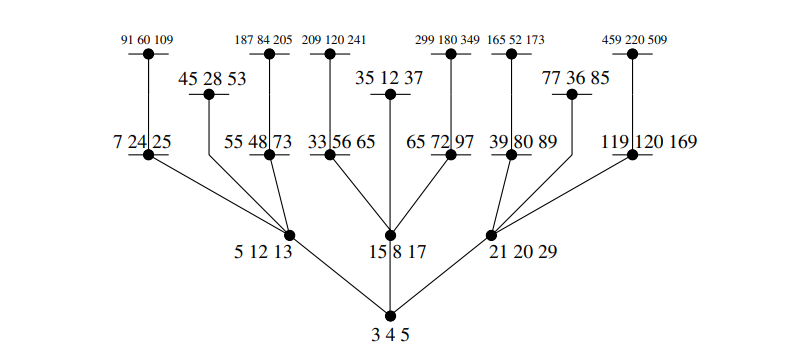
\includegraphics[scale=.5]{alperin_tree.png} 
\end{center}
\caption{Alperin's tree of Pythagorean triples.}
\label{farey diagram}
\end{figure}


\begin{lem}
 \textit{An integer matrix $X$ satisfies $X^2 = 0$ if and only if $X$ has the form}
\[
	X 
	= \begin{pmatrix} x & y \\ z & -x \end{pmatrix}
	= \begin{pmatrix}
mn & -n^2 \\
m^2 & -mn
\end{pmatrix}
= \begin{pmatrix} n \\ m \end{pmatrix} \begin{pmatrix} m & -n 
\end{pmatrix}	
\]
\textit{for integers $x$, $y$, and $z$ such that $x^2 + yz = 0$.}
\end{lem}




$$\begin{pmatrix} -y & x+z \\ x-z & y \end{pmatrix} $$
such that $x^2 + y^2 -z^2 = 0$.



\begin{table}[h]
% \centering
\renewcommand{\arraystretch}{2}
\begin{tabular}{|c|c|c|}
\hline
\multicolumn{3}{|c|}{\textbf{Magic Correspondence}} \\
\hline
 & Minkowski space $\mathbb{R}^{2,1}$ & Traceless $2 \times 2$ matrices \\
\hline
Main object & 
$\mathbf{v} = (x, y, z)$ & 
$\tilde{\mathbf{v}} = \sum v^i \sigma_i = \frac{1}{2}
\begin{pmatrix} -y & x+z \\ x-z & y \end{pmatrix}$ \\
\hline
Norm & 
$\|\mathbf{v}\| = -x^2 - y^2 + z^2$ & 
$\|\mathbf{v}\| = 4 \det \tilde{\mathbf{v}}$ \\
\hline
Action & 
$\mathbf{v}' = A\mathbf{v}$,\, \newline ($A \in O(2,1;\mathbb{Z})$) & 
$\tilde{\mathbf{v}}' = \tilde{A} \tilde{\mathbf{v}} \tilde{A}^*$,\, \newline ($\tilde{A} \in SL^{\pm}(2,\mathbb{Z})$) \\
\hline
Minkowski scalar product & 
$\mathbf{v} \cdot \mathbf{w} = \mathbf{v}^T G \mathbf{w}$ & 
$\mathbf{v} \cdot \mathbf{w} = -2 \mathrm{Tr}\,\tilde{\mathbf{v}} \tilde{\mathbf{w}}$ \\
\hline
The $i$th coefficient & 
$v^i = \mathbf{v} \cdot \mathbf{e}_i$ & 
$v^i = -\det \sigma_i \cdot \mathrm{Tr}(\tilde{\mathbf{v}} \sigma_1)$ \\
\hline
\end{tabular}
\caption{Correspondence between Minkowski space and traceless $2 \times 2$ matrices.}
\end{table}


\begin{table}[h]
% \centering
\renewcommand{\arraystretch}{2}
\begin{tabular}{|l|l|}
% \toprule
\textbf{Hyperbolic Geometry} & \textbf{Algebra/Number Theory} \\
\hline
horocycle & nonzero vector $(p,q) \in \mathbb{R}^2$ \\
	  % & &\\
\hline
geodesic & indefinite binary quadratic form $f$ \\
point & definite binary quadratic form $f$ \\
signed distance between horocycles & $2 \log \left| \det \begin{pmatrix} p_1 & p_2 \\ q_1 & q_2 \end{pmatrix} \right|$ \\
signed distance between horocycle & $\log \left( \dfrac{f(p,q)}{\sqrt{|\det f|}} \right)$ \\
% and geodesic/point & \\
% ideal triangulation of the modular torus & Markov triple \\
% \bottomrule
\end{tabular}
\caption{Correspondence between hyperbolic geometry and algebra/number theory.}
\end{table}

\thebibliography{99}

\bibitem{aigner2}
Aigner M., Ziegler G.M.  
\textit{Representing numbers as sums of two squares.} In: Proofs from THE BOOK. Springer, Berlin, Heidelberg. (2010)

\bibitem{alperin}
 R. C. Alperin, 
 The Modular Tree of Pythagoras,
 Amer. Math. Monthly 112 (2005), 807–816
 \url{https://web.archive.org/web/20231014013915/http://www.math.sjsu.edu/%7Ealperin/pt.pdf}

\bibitem{conway}
Conway, J. H. and Guy, R. K. \textit{Farey Fractions and Ford
Circles.} The Book of Numbers. New York: Springer-Verlag, pp. 152-154, 1996.

\bibitem{dolan}
Dolan, S., 
\textit{A very simple proof of the two-squares theorem.}
The Mathematical Gazette, 106(564), 511-511. (2021) doi:10.1017/mag.2021.120

\bibitem{elsholtz}
Elsholtz C.A 
\textit{Combinatorial Approach to Sums of Two Squares and Related Problems.}
 In: Chudnovsky D., Chudnovsky G. (eds) Additive Number Theory. Springer, New York, NY.
 (2010) 


\bibitem{ford}
Ford, L. R.,  \textit{Fractions.} Amer. Math. Monthly, 45, (9), 586–601 (1938).



\bibitem{heath}
Heath-Brown, Roger. 
\textit{ Fermat’s two squares theorem.} Invariant (1984) 



\bibitem{vlad}
Greg McShane, Vlad Sergiescu,
\textit{Geometry of Fermat's sum of squares}
\url{https://macbuse.github.io/squares.pdf}

\bibitem{macbuse}
Github repo FAREY DIAGRAM \url{https://github.com/macbuse/FAREY_DIAGRAM}

\bibitem{bob}
R. C. Penner, 
\textit{The decorated Teichmueller space of punctured surfaces}, 
Communications in Mathematical Physics 113 (1987), 299–339.


% \bibitem{north}
% Northshield, Sam. 
% \textit{A Short Proof of Fermat’s Two-square Theorem.} The American Mathematical Monthly. 127. 638-638. (2020). 

\bibitem{serre}
J-P. Serre,
\textit{A Course in Arithmetic},
Graduate Texts in Mathematics,
Springer-Verlag New York
1973


% \bibitem{series}
% Series, C. (1985), 
% \textit{The Modular Surface and Continued Fractions. Journal of the London} Mathematical Society, s2-31: 69-80. 

\bibitem{springborn1}
B. Springborn. The hyperbolic geometry of Markov’s theorem on Diophantine
approximation and quadratic forms. Enseign. Math., 63(3-4):333–373, 2017.

\bibitem{springborn2}
Boris Springborn,
\textit{The worst approximable rational numbers}
\url{https://arxiv.org/abs/2209.15542}



\bibitem{zagier}
D. Zagier,
 \textit{A one-sentence proof that every prime p = 1 (mod 4) is a sum of two squares}, 
 American Mathematical Monthly, 97 (2): 144

 \bibitem{copilot}
 Github Copilot \url{https://copilot.github.com/}

 \bibitem{vim_copilot}
Tim Pope, copilot.vim \url{https://github.com/github/copilot.vim}
 

\bibitem{mathews}
Daniel V. Mathews,
\textit{Spinors and horospheres}
\url{https://arxiv.org/abs/2308.09233}

\bibitem{katayama}
 Shin-ichi Katayama. Modified farey trees and pythagorean triples.
 Journal of mathematics, the University of Tokushima, 47, 2013.
 \url{https://scispace.com/pdf/modified-farey-trees-and-pythagorean-triples-kxeavtdvnr.pdf}

\bibitem{kocik1}
Jerzy Kocik,
\textit{Clifford Algebras and Euclid's Parameterization of Pythagorean Triples},
Advances in Applied Clifford Algebras 17 (2007), 71-93.
\url{https://arxiv.org/abs/1201.4418}

\bibitem{hall}
 A. Hall, 
 Genealogy of Pythagorean triads, 
 Mathematical Gazette, LIV, No. 390
(1970), 377–379.

\bibitem{hall2}
Keith Conrad
Pythagorean descent
\url{https://kconrad.math.uconn.edu/blurbs/linmultialg/descentPythag.pdf}


 \bibitem{lee}
H. Lee Price
 The Pythagorean Tree: A New Species
 \url{https://arxiv.org/abs/0809.4324}

 \bibitem{zimhoni}
Noam Zimhoni,
 A forest of eisensteinian triplets
The American Mathematical Monthly
Vol. 127, No. 7 , pp. 629-637 \url{https://arxiv.org/abs/1904.11782}



\end{document}
